In order to make comparisons even fairer , the code about the application's core and about the UI is shared between different solution. In this way , measurements are taken considering only the parts of the code added by each solution's implementation. This subsection presents the shared parts in details. Some parts of the code can change from one implementation to another in order to adapt to the solution's pattern. However, changes to the structure are kept minimal and the same is for the UI. It uses the least widgets and visual elements possible. In  Figure \ref{fig:todo_app_shared_folder_structure} the shared folder's and file's structure is shown. Subsequent paragraphs exaplain how models, pages, components and the repository are implemented. 

		
		\begin{figure}[H]
		    \centering
		    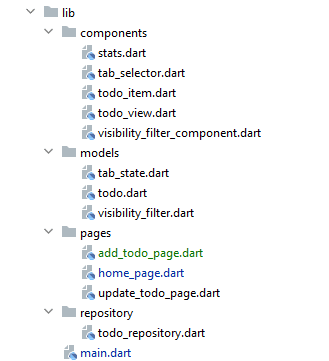
\includegraphics[width=0.6\textwidth]{Images/folder_structure.png}
		    \caption{Shows Todos app's shared files structure}
		    \label{fig:todo_app_shared_folder_structure}
		\end{figure}
		
		
		
\paragraph{The application's Root - }
		\label{par:todo_app_application_root}
The root widget of the application is called MyApp.
It is a stateless widget composed by a MaterialApp widget. Inside the MaterialApp widget, three routes are defined : the HomePage , the UpdateTodoPage and the AddTodoPage. The \textit{inizialRoute} is set to the HomePage as deafult. The UpdateTodoPage takes a Todo instance as argument. Inside the \textit{main} function the MyApp widget is passed to the \textit{runApp} method in order to start the application.

		\begin{code}
		\captionof{listing}{Todo app - MaterialApp and main function implementation} 
		\label{code:2.1}
	\begin{minted}[bgcolor=bluepoli!10]{dart}
	
void main() {
  //launching the application
  runApp(const MyApp());
}

class MyApp extends StatelessWidget {
  const MyApp({Key? key}) : super(key: key);

  @override
  Widget build(BuildContext context) {
    return MaterialApp(
      initialRoute: "/", //setting initial route to the HomePage
      routes: { //defining possible routes
        "/": (context) => const HomePage(),
        "/updateTodo": (context) => UpdateTodoPage(
              todo: (ModalRoute.of(context)!.settings.arguments
                      as Todo),
        "/addTodo": (context) => AddTodoPage(),
      },
    );
  }
}
	\end{minted}
\end{code}	
	
	\paragraph{Models - }
	\label{par:todo_app_models_and_repository}
The model for the HomePage's tabs is implemented using an enumeration.

	\begin{code}
	\captionof{listing}{Todo app - TabState model implementation}
			\label{code:2.2}
	\begin{minted}[bgcolor=bluepoli!10]{dart}
enum TabState{
	todos,stats
}
	\end{minted}
	\end{code}

Filters for the \textit{filteredTodos} list are modelled by an enumeration too. They can take three values: \textit{all, notCompleted, completed}.
\begin{code}	
	\captionof{listing}{Todo app - VisibilityFilter model implementation}
			\label{code:2.3}
	\begin{minted}[bgcolor=bluepoli!10]{dart}
enum VisibilityFilter{
	completed,notCompleted,all
}
	\end{minted}
	\end{code}
	
It's not possible to give a common implementation for the Todo model matching every solution. Todo model, indeed, can change in different implementations. The sharable structure of the model, however, can defined as shown in Source Code \ref{code:2.4}
	\mbox{}\\
	\begin{code}
	
	\captionof{listing}{Todo app - Todo model implementation} 
\label{code:2.4}
	\begin{minted}[bgcolor=bluepoli!10]{dart}
	
@immutable
class Todo {
  final int id;
  final String name;
  final String description;
  final bool completed;

  const Todo(
      {required this.id,
      required this.name,
      required this.description,
      required this.completed});

  @override
  bool operator ==(Object other) {
    return (other is Todo) &&
        other.description == description &&
        other.name == name &&
        other.id == id &&
        other.completed == completed;
  }

  @override
  String toString() {
    return "{ id: $id  completed: $completed}";
  }

  @override
  // TODO: implement hashCode
  int get hashCode => super.hashCode;
}

	\end{minted}
	\end{code}
	
\paragraph{Repository and utilities - }
	\label{par:todo_app_models_and_repository}
Some useful functions are shared between different implementations. They are contained in the utility.dart file. \textit{generateId} function takes a list of todos and generate a new unique id. \textit{todoExists} function takes a list of todos and a id and checks if a todo with that id exists.
\mbox{}\\
\begin{code}
	\captionof{listing}{Todo app - Utility functions implementation} 
			\label{code:2.5}
	\begin{minted}[bgcolor=bluepoli!10]{dart}
	
int generateId(List<Todo> todos) {
  Random rand = Random();
  int newInt = rand.nextInt(1000) + 2;
  List<int> ids = todos.map((todo) => todo.id).toList();
  while (ids.contains(newInt)) {
    newInt = rand.nextInt(1000) + 2;
  }
  return newInt;
}

bool todoExists(List<Todo> todos, int id) {
  List<Todo> result = todos.where((todo) => todo.id == id).toList();
  return result.isNotEmpty ? true : false;
}
	\end{minted}
	\end{code}
The TodoRepository class simulates the todos's fetching process from a Database. It has two static methods. These methods are asynchronous and have a duration of 2 seconds to give the impression of a real asynchronous operation. The method \textit{loadTodos}, in particular, populates a list with six new todo instances, using the \textit{generateId} function for the generation of their unique IDs. Subsequently, 2 seconds later, it returns the list to the caller.
	\mbox{}\\
	\begin{code}
	\captionof{listing}{Todo app - TodoRepository implementation} 
			\label{code:2.6}
	\begin{minted}[bgcolor=bluepoli!10]{dart}
	
class TodoRepository {
  //generate 6 unique todos
  static Future<List<Todo>> loadTodos() async {
    List<Todo> todos = [];
    Random rand = Random();
    while (todos.length < 6) {
      int newInt = generateId(todos);
      todos.add(Todo(
          id: newInt,
          name: "Todo " + newInt.toString(),
          description: "description " + newInt.toString(),
          completed: rand.nextBool()));
    }
//waiting 2 seconds before returning the list
    await Future.delayed(const Duration(seconds: 2));
    return todos;
  }

  static Future<void> saveTodos(List<Todo> todos) async {
    await Future.delayed(const Duration(seconds: 2));
  }
}
	\end{minted}
	\end{code}
	
	\paragraph{Components - } 
	\label{par:todo_app_components}
	Components are widgets created with a specific task. They provide some sort of indipendent functionality.
	TodoView widget component, for example, takes care of visualizing a list of todos. Todos are accessed in different ways depending on the implementation. TodoView widget uses a ListView widget filled with TodoItem widgets. \textit{itemCount} and \textit{itemBuilder} fields are left empty for future implementation.
\mbox{}
	\begin{code}
	\captionof{listing}{Todo app - TodoView component implementation} \mbox{}
			\label{code:2.7}
	\begin{minted}[bgcolor=bluepoli!10]{dart}
	class TodoView extends StatelessWidget {
	
	  const TodoView({Key? key}) : super(key: key);
	
	  @override
	  Widget build(BuildContext context) {
	    print("Building TodoView");
	
	    return ListView.builder(
	      itemCount: //to be filled,
	      itemBuilder: (context, index) {
	        return TodoItem(
	        todo: //to be filled 
	        );
	      },
	    );
	  }
	}
	\end{minted}
	\end{code}

TodoItem widget component takes care of visualizing a specific todo. TodoItem widget is a stateless. It uses two Text widgets in order to display the todo's informations and a Checkbox widget to allow changing the todo’s \textit{completed} field. The entire TodoItem widget is wrapped into an InkWell widget to make it responsive to taps. Functions fields are left empty for future implementation.
	
	\mbox{}
	\begin{code}
	\captionof{listing}{Todo app - TodoItem component implementation} \mbox{}
			\label{code:2.8}
	\begin{minted}[bgcolor=bluepoli!10]{dart}
class TodoItem extends StatelessWidget {
  final Todo todo;

  const TodoItem({Key? key, required this.id}) : super(key: key);

  @override
  Widget build(BuildContext context) {
    print("Building Todo Item \$todo");

    return InkWell(
      onTap: () {
        Navigator.pushNamed(context, "/updateTodo" , arguments: todo);
      },
      child: Row(
        children: [
          Column(
            children: [
              Text(todo.name,
                  style: const TextStyle(fontSize: 14,
                   color: Colors.black)),
              Text(todo.description,
                  style: const TextStyle(fontSize: 10,
                   color: Colors.grey)),
            ],
          ),
          Checkbox(
              value: todo.completed,
              onChanged: (value) {
              //to be filled
              }),
        ],
      ),
    );
  }
}

	\end{minted}
	\end{code}	
TabSelector component allows to switch from tabs. It uses a BottomNavigationBar widget. Its \textit{items} field is populated with a list of BottomNavigationBarItem widgets that comes from the mapping of all possible TabState values to BottomNavigationBarItem widgets. Function fields are left empty for future implementation.
	 Functions fields are left empty for future implementation.
	
	\mbox{}
	\begin{code}
	\captionof{listing}{Todo app - TabSelector component implementation} \mbox{}
			\label{code:2.9}
	\begin{minted}[bgcolor=bluepoli!10]{dart}
class TabSelector extends StatelessWidget {

  const TabSelector(
      {Key? Key})
      : super(key: key);

  @override
  Widget build(BuildContext context) {
    print("Building Tab Selector");

    return BottomNavigationBar(
      currentIndex: //to be filled ,
      onTap: (){
      //to be filled
      },
      items: TabState.values
          .map((tab) => BottomNavigationBarItem(
                label: describeEnum(tab),
                icon: Icon(
                  tab == TabState.todos ? Icons.list : Icons.show_chart,
                ),
              ))
          .toList(),
    );
  }
}

	\end{minted}
	\end{code}
VisibilityFilterSelector component uses a DropdownButton widget. Its \textit{items} field is populated with a list of DropdownMenuItem widgets that comes from the mapping of all possible VisibilityFilter values to DropdownMenuItem widgets. Function fields are left empty for future implementation.
	
	\mbox{}
	\begin{code}
\captionof{listing}{Todo app - VisibilityFilterSelector component implementation} \mbox{}
		\label{code:2.10}
\begin{minted}[bgcolor=bluepoli!10]{dart}
class VisibilityFilterSelector extends StatelessWidget {

  const VisibilityFilterSelector(
      {Key? key})
      : super(key: key);

  @override
  Widget build(BuildContext context) {
    print("Building Visibility filter");
    
    return DropdownButton<VisibilityFilter>(
      value: //to be filled,
      items: VisibilityFilter.values.map((filter) {
        return DropdownMenuItem<VisibilityFilter>(
            child: Text(describeEnum(filter)), value: filter);
      }).toList(),
      onChanged: (filter) {
       //to be filled
      },
    );
  }
}

	\end{minted}
	\end{code}

Stats component takes care of visualizing some numerical representation regarding the list of todos. Stats component is a stateless widget composed by a Text widget, showing the stats value, wrapped into a Center widget.
	
	\mbox{}
	\begin{code}
	\captionof{listing}{Todo app - Stats component implementation} \mbox{}
		\label{code:2.11}
	\begin{minted}[bgcolor=bluepoli!10]{dart}
class Stats extends StatelessWidget {
  const Stats({Key? key}) : super(key: key);

  @override
  Widget build(BuildContext context) {
    print("Building Stats");

    return Center(
        child: Text(
	// to be filled        
        ));
  }
}
	\end{minted}
	\end{code}
	\paragraph{Pages - } 
	\label{par:todo_app_pages}
The HomePage can be a statefull widget or a stateless  widget depending on the utilized solution. In both cases it uses a simple Scaffold widget. The AppBar widget contains a VisibilityFilterSelector component only when the tab is set to \textit{todos}. The \textit{body} is filled with a TodoView component if the tab is set to \textit{todos} and with a Stats component if the tab is set to \textit{stats}. The \textit{body} can change from \textit{todos} tab to \textit{stats} tab using the BottomNaviagationBar (filled with the TabSelector widget). An empty FloatingActionButton widget is also present for future implementation.
	(note: some small pieces could change in different solution’s implementation. In the above example the tab value is contained in the HomePage but it will not be always the case).

	\mbox{}
	\begin{code}
	\captionof{listing}{Todo app - HomePage implementation} \mbox{}
			\label{code:2.12}

	\begin{minted}[bgcolor=bluepoli!10]{dart}

class HomePage extends StatefulWidget {
  const HomePage({Key? key}) : super(key: key);

  @override
  State<HomePage> createState() => _HomePageState();
}

class _HomePageState extends State<HomePage> {
  TabState tab = TabState.todos; //example of tab handling

  @override
  Widget build(BuildContext context) {
        return Scaffold(
          appBar: AppBar(
            actions: [
              tab == TabState.todos
                  ? const VisibilityFilterComponent()
                  : Container()
            ],
            title: const Text("Todo App"),
          ),
          body: tab == TabState.todos ? const TodoView() : const Stats(),
          bottomNavigationBar: TabSelector(),
          floatingActionButton: tab == TabState.todos
              ? FloatingActionButton(
                  child: const Icon(Icons.plus_one),
            onPressed: () {
              Navigator.pushNamed(context, "/addTodo");

            },
          ) : Container(),
        );
  }
}
	\end{minted}
	\end{code}

The UpdateTodoPage is statefull and uses a Scaffold widget too. The reason why it is implemented with a statefull widget is that it uses TextEditingController objects which need a statefull widget to work properly. The \textit{body} is filled with a Column widget containing two TextField widgets and a TextButton widget. The TextButton widget \textit{onPressed }field is left empty for future implementation.
	\mbox{}\\
	\begin{code}
	\captionof{listing}{Todo app - UpdateTodoPage implementation} \mbox{}
			\label{code:2.13}
	\begin{minted}[bgcolor=bluepoli!10]{dart}

class UpdateTodoPage extends StatefulWidget {
  final Todo todo;

  const UpdateTodoPage({Key? key, required this.todo})
      : super(key: key);

  @override
  State<UpdateTodoPage> createState() => _UpdateTodoPageState();
}

class _UpdateTodoPageState extends State<UpdateTodoPage> {
  final textControllerName = TextEditingController();
  final textControllerDesc = TextEditingController();

  @override
  Widget build(BuildContext context) {
    return Scaffold(
        appBar: AppBar(
          title: Text("Update Todo" + widget.todo.name),
        ),
        body: Column(
          children: [
            TextField(
              controller: textControllerName,
              decoration: const InputDecoration(
                  border: OutlineInputBorder(), 
                  hintText: 'Enter a new name'),
            ),
            TextField(
              controller: textControllerDesc,
              decoration: const InputDecoration(
                  border: OutlineInputBorder(),
                  hintText: 'Enter a new description'),
            ),
            TextButton(
                onPressed: () {
                  //to be filled
                },
                child: const Text("Confirm"))
          ],
        ));
  }

  @override
  void dispose() {
    textControllerName.dispose();
    textControllerDesc.dispose();
    super.dispose();
  }
}

	\end{minted}
	\end{code}

The AddTodoPage is statefull and uses a Scaffold widget. The \textit{body} field is filled with a Column widget containing two TextField widgets and a TextButton widget. The TextButton \textit{onChanged }field is left empty for future implementation.
	\mbox{}
	\begin{code}
	\captionof{listing}{Todo app - AddTodoPage implementation} \mbox{}
			\label{code:2.14}
	\begin{minted}[bgcolor=bluepoli!10]{dart}

class AddTodoPage extends StatefulWidget {

  const AddTodoPage({Key? key, required})
      : super(key: key);

  @override
  State<AddTodoPage> createState() => _AddTodoPageState();
}

class _AddTodoPageState extends State<AddTodoPage> {
  final textControllerName = TextEditingController();
  final textControllerDesc = TextEditingController();

  @override
  Widget build(BuildContext context) {
    return Scaffold(
        appBar: AppBar(
          title: const Text("Add Todo"),
        ),
        body: Column(
          children: [
            TextField(
              controller: textControllerName,
              decoration: const InputDecoration(
                  border: OutlineInputBorder(), hintText: 'Enter a name'),
            ),
            TextField(
              controller: textControllerDesc,
              decoration: const InputDecoration(
                  border: OutlineInputBorder(),
                  hintText: 'Enter a description'),
            ),
            TextButton(
                onPressed: () {
                  //to be filled
                },
                child: const Text("Create"))
          ],
        ));
  }

  @override
  void dispose() {
    textControllerName.dispose();
    textControllerDesc.dispose();
    super.dispose();
  }
}

	\end{minted}
	\end{code}
Here ends the implementation of the shared code.